% abtex2-modelo-artigo.tex, v-1.9.2 laurocesar
% Copyright 2012-2014 by abnTeX2 group at http://abntex2.googlecode.com/ 
%

% ------------------------------------------------------------------------
% ------------------------------------------------------------------------
% abnTeX2: Modelo de Artigo Acadêmico em conformidade com
% ABNT NBR 6022:2003: Informação e documentação - Artigo em publicação 
% periódica científica impressa - Apresentação
% ------------------------------------------------------------------------
% ------------------------------------------------------------------------


% ------------------------------------------------------------------------
% Modelo de pré-projeto para TCC 
% Universidade Federal do Piauí - CSHNB
% ------------------------------------------------------------------------



\documentclass[
	% -- opções da classe memoir --
	article,			% indica que é um artigo acadêmico
	11pt,				% tamanho da fonte
	oneside,			% para impressão apenas no verso. Oposto a twoside
	a4paper,			% tamanho do papel. 
	% -- opções da classe abntex2 --
	%chapter=TITLE,		% títulos de capítulos convertidos em letras maiúsculas
	%section=TITLE,		% títulos de seções convertidos em letras maiúsculas
	%subsection=TITLE,	% títulos de subseções convertidos em letras maiúsculas
	%subsubsection=TITLE % títulos de subsubseções convertidos em letras maiúsculas
	% -- opções do pacote babel --
	english,			% idioma adicional para hifenização
	brazil,				% o último idioma é o principal do documento
	sumario=tradicional
	]{abntex2}


% ---
% PACOTES
% ---

% ---
% Pacotes fundamentais 
% ---
\usepackage{lmodern}			% Usa a fonte Latin Modern
\usepackage[T1]{fontenc}		% Selecao de codigos de fonte.
\usepackage[utf8]{inputenc}		% Codificacao do documento (conversão automática dos acentos)
\usepackage{indentfirst}		% Indenta o primeiro parágrafo de cada seção.
\usepackage{nomencl} 			% Lista de simbolos
\usepackage{color}				% Controle das cores
\usepackage{graphicx}			% Inclusão de gráficos
\usepackage{microtype} 			% para melhorias de justificação

% ---
		
% ---
% Pacotes adicionais, usados apenas no âmbito do Modelo Canônico do abnteX2
% ---
\usepackage{lipsum}				% para geração de dummy text
% ---
		
% ---
% Pacotes de citações
% ---
\usepackage[brazilian,hyperpageref]{backref}	 % Paginas com as citações na bibl
\usepackage[alf]{abntex2cite}	% Citações padrão ABNT
% ---

% ---
% Configurações do pacote backref
% Usado sem a opção hyperpageref de backref
\renewcommand{\backrefpagesname}{Citado na(s) página(s):~}
% Texto padrão antes do número das páginas
\renewcommand{\backref}{}
% Define os textos da citação
\renewcommand*{\backrefalt}[4]{
	\ifcase #1 %
		Nenhuma citação no texto.%
	\or
		Citado na página #2.%
	\else
		Citado #1 vezes nas páginas #2.%
	\fi}%
% ---

% ---
% Informações de dados para CAPA e FOLHA DE ROSTO
% ---
\titulo{Avaliação de Segurança de Redes sem Fio com Foco em WPS}
\autor{
	Aluno: Carlos Daniel da Silveira Santos (MATRÍCULA:20189022361)
	\\
	E-mail: cdanielss1973@outlook.com; Período da Graduação: VI
	\\
	Orientador: Fredison Muniz de Sousa
}
% ---

% ---
% Configurações de aparência do PDF final

% alterando o aspecto da cor azul
\definecolor{blue}{RGB}{41,5,195}

% informações do PDF
\makeatletter
\hypersetup{
     	%pagebackref=true,
		pdftitle={\@title}, 
		pdfauthor={\@author},
    	pdfsubject={Modelo de artigo científico com abnTeX2},
	    pdfcreator={LaTeX with abnTeX2},
		pdfkeywords={abnt}{latex}{abntex}{abntex2}{atigo científico}, 
		colorlinks=true,       		% false: boxed links; true: colored links
    	linkcolor=blue,          	% color of internal links
    	citecolor=blue,        		% color of links to bibliography
    	filecolor=magenta,      		% color of file links
		urlcolor=blue,
		bookmarksdepth=4
}
\makeatother
% --- 

% ---
% compila o indice
% ---
\makeindex
% ---

% ---
% Altera as margens padrões
% ---
\setlrmarginsandblock{3cm}{3cm}{*}
\setulmarginsandblock{3cm}{3cm}{*}
\checkandfixthelayout
% ---

% --- 
% Espaçamentos entre linhas e parágrafos 
% --- 

% O tamanho do parágrafo é dado por:
\setlength{\parindent}{1.3cm}

% Controle do espaçamento entre um parágrafo e outro:
\setlength{\parskip}{0.2cm}  % tente também \onelineskip

% Espaçamento simples
\SingleSpacing

% ----
% Início do documento
% ----
\begin{document}

% Retira espaço extra obsoleto entre as frases.
\frenchspacing 

% ----------------------------------------------------------
% ELEMENTOS PRÉ-TEXTUAIS
% ----------------------------------------------------------

% página de titulo
\maketitle

% resumo em português
\begin{resumoumacoluna}
\textbf{Contexto:} 
O \textit{Wi-Fi Protected Setup} (WPS) é um padrão definido pela Wi-Fi AllianceTM, para segurança de redes sem fio (Wi-Fi). Foi introduzido em 2006 e vinha para fornecer uma configuração mais fácil e substituir padrões obsoletos. Apesar de trazer novas funcionalidades, também trouxe consigo algumas vulnerabilidades. Como a principal falha do WPS, que é ser composto por um PIN (Número de identificação pessoal) de apenas 8 dígitos, suscetível a ataques de força bruta.

\textbf{Problema:}
Com o avanço e o grande aumento dos serviços online, as redes de computadores estão cada vez mais vulneráveis. 
Hoje, quase todos os computadores e dispositivos móveis estão conectados à grande rede da Internet, onde problemas podem ocorrer, seja por próprio descuido do usuário, deixando sua máquina exposta ou por falhas de segurança da rede. Por isso, faz-se necessário o estudo das vulnerabilidades e falhas dos equipamentos de redes, para uma utilização adequada de acordo com o usuário.

\indent
\textbf{Proposta:}
Este pré-projeto visa avaliar redes domésticas que estão vulneráveis, principalmente por conta do protocolo WPS, utilizando como cenário o município de Picos do Estado do Piauí (Picos - PI). 
A coleta de dados será feita com o auxílio do método de \textit{WarDriving}, para a captura e análise de dados como: Protocolos de Segurança e configurações WPS.  
A análise dos dados visa contribuir para o desenvolvimento de métodos sistemáticos que possam auxiliar no desenvolvimento de novas soluções de segurança. 


 \vspace{\onelineskip}
 
 \noindent
\textbf{Palavras-chaves}: Wi-Fi, WPS, Segurança, Internet, Protocolo.

\end{resumoumacoluna}

% ]  				% FIM DE ARTIGO EM DUAS COLUNAS
% ---

% ----------------------------------------------------------
% ELEMENTOS TEXTUAIS
% ----------------------------------------------------------
\textual

% ----------------------------------------------------------
% Introdução
% ----------------------------------------------------------
\section{Introdução}
As redes de computadores são formadas por computadores autônomos que trocam informações entre si. Essa conexão pode ser feita de várias formas como fios de cobre, fibra óptica e ondas de rádio. Nestes sistemas são utilizados equipamentos concentradores denominados \textit{switches}, para interligação dos computadores em uma rede e cliente-servidor que é uma estrutura que distribui as tarefas entre os fornecedores de um recurso (servidores) e os requerentes dos serviços (clientes) \cite{tanenbaum2011redes}. 

A estrutura de uma rede conta com uma estrutura lógica para se comunicar, denominada protocolo de comunicação. Os protocolos são conjuntos de regras que visam estabelecer a comunicação entre as camadas do modelo OSI (\textit{Open Systems Interconnection}). Os mesmos realizam o controle do formato e o significado das informações passadas \cite{tanenbaum2011redes}. O \textit{Wi-Fi Protected Setup} (WPS) é usado como padrão de segurança para redes sem fio (Wi-Fi), que visa fazer a conexão entre um dispositivo e uma rede sem fio de maneira rápida e fácil. Essa tecnologia funciona em redes sem fio com uma senha criptografada.

Embora o WPS seja comercializado como uma forma segura de configurar um dispositivo sem fio, existem projetos e falhas de implementação que permitem a um invasor obter acesso a uma rede sem fio protegida \cite{viehbock2011brute}. As duas das principais formas de atacar um dispositivo Wi-Fi com WPS são: A primeira é um ataque de força bruta offline que usa desequilíbrio no registro do protocolo. Este ataque requer ação do usuário, mas é o mais eficiente. A segunda forma de ataque usa fraquezas no implementação de WPS e fornece um \textit{evil twin}. Este ataque mostra que mesmo desabilitando completamente o WPS nos roteadores, todas as vulnerabilidades não são cobertas \cite{mohtadi2015new}.

\subsection{Objetivos Gerais e Específicos}
O objetivo geral deste pré-projeto é levantar dados que mostrem o atual cenário do nível de segurança das redes Wi-Fi no município de Picos do Estado do Piauí (Picos - PI). Os objetivos específicos deste trabalho são:
\begin{itemize}
   \item Identificar o perfil das redes Wi-Fi da cidade de Picos;
   \item Demonstrar o atual nível de segurança das redes identificadas; 
   \item Criar métodos sistemáticos que auxiliem na segurança das redes Wi-Fi.
\end{itemize}

\section{Justificativa}
A tecnologia das redes sem fio obteve um grande salto na quantidade de utilizadores pela conveniência e praticidade na utilização dos dispositivos móveis \cite{tanenbaum2011redes}. Dessa forma, criaram-se novos riscos aos dispositivos e usuários e consequentemente novos desafios às empresas desenvolvedoras. Portanto foram necessários investimentos para o desenvolvimento de tecnologias que aliem mais segurança e qualidade na utilização dessas redes.

O interesse no assunto surgiu da necessidade de entender os riscos a que as pessoas estão expostas ao utilizar as redes sem fio e de verificar se existe algum mecanismo que realmente garantam a segurança neste ambiente. Diversas tecnologias são desenvolvidas e adicionadas às redes sem fio para melhorar a experiência do usuário final, permitindo que este possa, por exemplo, instalar um roteador \textit{wireless} em casa e conectar seus dispositivos com pouco ou nenhum conhecimento técnico \cite{silva2014vulnerabilidade}.

Diante da grande quantidade de usuários das redes sem fio, e tendo as mais diversas formas de ataques a vulnerabilidades, é necessário uma utilização consciente das ferramentas e dispositivos, pois a segurança é necessária em várias camadas de uma arquitetura de rede para proteção contra atacantes, que têm à mão um grande arsenal de ataques possíveis \cite{kurose2007redes}. Uma boa alternativa para lidar com os tais problemas seria sempre a atualização do software do dispositivo e uma configuração apropriada.

Mantendo o WPS ativo pode ser um fator de risco alto, ou seja, permitir um acesso não autorizado na rede e possivelmente  ao restante do ambiente, quer seja para usá-lo como ponte para outros ambientes, quer seja para capturar informações que trafegam para outros ambientes 
Wi-Fi. Mesmo que a senha não seja exposta, e o PIN do WPS for descoberto já é suficiente para ter acesso a rede \cite{rufino2019segurancca}.

O presente trabalho visa solucionar um dos grandes problemas, para se desenvolver soluções por meio de métodos sistemáticos, para a segurança de redes. Sendo ele a falta de informações sobre o estado da rede. Além de fornecer conhecimentos na aplicação das contramedidas de segurança necessárias para mitigar os riscos e uma utilização devida dos equipamentos.

\section{Referencial Teórico}
Esta Seção apresenta os conceitos fundamentais para a compreensão do pré-projeto. Na Subseção \ref{sec:wifi} descreve as Redes sem Fios, abordando os seus conceitos de criação. Já a Subseção \ref{sec:protocolo} contextualiza sobre os protocolos, adentrando nas falhas e vulnerabilidades. 

\subsection{Redes sem Fios}
\label{sec:wifi}
A tecnologia \textit{wireless} significa “sem fio” (em livre tradução), e possibilita a transmissão da conexão entre pontos distantes sem precisar usar fios (como telefones sem fio, rádios ou o seu celular) \cite{cancelaimportancia}. Essa tecnologia engloba uma série de outras, sendo a mais comum delas a Wi-Fi. Podem ser consideradas \textit{wireless}, como o IrDA (\textit{Infrared Data Association}) que transmite através de um adaptador infravermelho, há também o \textit{bluetooth} muito utilizado em \textit{smartphones}, porém sua distância é relativamente curta, dentre outros \cite{engst2005kit}.

O \textit{Institute of Electrical and Electronic Engineers} (IEEE) constituiu um grupo de pesquisa para criar padrões abertos que pudessem tornar a tecnologia sem fio cada vez mais realidade, tendo como objetivo desenvolver padrões técnicos de acordo com fabricante, definindo como dará a comunicação entre fabricante e cliente de rede. Ao longo do tempo, foram desenvolvidos diversos padrões, a qual destacou e melhor desenvolveu foi o padrão 802.11, conhecido como Wi-Fi (\textit{Wireless Fidelity} ou fidelidade sem fio) \cite{rufino2019segurancca}.

O comitê apresentou o padrão IEEE 802.11 que foi inicialmente definido como uma especificação de nível físico e de \textit{enlace} do modelo OSI para redes locais sem fio WLAN. A WLAN  funcionava a 1 Mbps (megabits por segundo) ou 2 Mbps \cite{tanenbaum2003redes}. Com o passar do tempo outros padrões foram criados, de acordo com a necessidade do mercado, o último padrão apresentado é o 802.11ax, que foi ratificado no segundo semestre de 2019, vindo para fornecer um desempenho mais previsível para aplicações avançadas, como vídeo 4K ou 8K \cite{lopez2019ieee}. 

\subsection{Protocolos de Segurança}
\label{sec:protocolo}
Todas as atividades na \textit{Internet} que envolvem duas ou mais entidades remotas comunicantes são governadas por um protocolo. Por exemplo, protocolos executados no hardware de dois computadores conectados fisicamente controlam o fluxo de bits no “cabo” entre as duas placas de interface de rede; protocolos de controle de congestionamento em sistemas finais controlam a taxa com que os pacotes são transmitidos entre a origem e o destino; protocolos em roteadores determinam o caminho de um pacote da origem ao destino \cite{kurose2007redes}.


\subsubsection{Protocolo WEP (\textit{Wired Equivalent Privacy})}
O protocolo IEEE 802.11 WEP foi criado em 2009 para fornecer autenticação e criptografia de dados entre um hospedeiro e um ponto de acesso sem fio (ou seja, a estação-base) usando uma técnica de chave compartilhada simétrica. A WEP não especifica um algoritmo de gerenciamento de chave, então supomos que o hospedeiro
e o ponto de acesso sem fio de alguma forma concordam sobre a chave através de um método fora da banda \cite{kurose2007redes}.

O WEP trabalha com chaves simétricas, ou seja, a mesma chave é sempre
utilizada para encriptar e desencriptar as informações que serão trafegadas na rede. O WEP possui uma série de problemas e a incapacidade de garantir a confidencialidade dos dados neste protocolo foi comprovada em \cite{fluhrer2001weaknesses}. O WEP pode ser quebrado através de ataques probabilísticos que foram otimizados em diversos programas específicos para isso (como o software \textit{WEPCrack} e \textit{Airsnort}). O atacante necessita capturar alguns milhares de pacotes e executar a análise via software para obter o segredo compartilhado.


\subsubsection{Protocolo WPA (Wi-Fi \textit{Protected Access})}
Para corrigir as vulnerabilidades apontadas no WEP, foi criado o WPA, protocolo de criptografia mais robusta do que o anterior. A criação do WPA tinha como o foco manter a compatibilidade com o WEP, mas ampliando suas características de segurança. O WPA não fornece apenas criptografia de dados forte para corrigir os pontos fracos do WEP, ele adiciona autenticação do usuário que estava faltando WEP \cite{alliance2003wi}.

Com o WPA foi apresenta uma nova tecnologia de chave denominada TKIP (\textit{Temporal Key Integrity Protocol}), na qual a chave de criptografia é trocada periodicamente, sua autenticação é por trocas de chaves dinâmicas, prevenindo ataques de retransmissão de pacotes. Mesmo diante dessas melhorias do WPA, se um atacante obtiver os quadros trocados durante o processo de autenticação, é possível que realize um ataque de força bruta \cite{fleishman2003weakness}. 
 
 
\subsubsection{Protocolo WPA2 (Wi-Fi \textit{Protected Access2})}
O protocolo WPA2 foi desenvolvido para a obtenção de um nível de segurança ainda maior que no padrão WPA, que para isso substitui o método criptográfico do WPA \cite{stangarlin2017analise}. O WPA2 introduz um novo algoritmo criptográfico, que é considerado completamente seguro, mas traz o inconveniente de não poder se comunicar com algumas interfaces de rede mais antigas. O WPA2 é considerado o padrão de segurança Wi-Fi mais seguro, pois apresenta componentes que são cruciais para a segurança da rede
sem fio, Autenticação, Cifragem e Integridade \cite{kumar2014literature}. 

Porém mesmo sendo considerado o padrão de segurança mais seguro, o WPA2 não está livre de falhas, foi constatada uma falha batizada de KRACK (\textit{Key Reinstallation Attacks}) que expôs quase todas as redes \textit{wireless}. O ataque consiste em enganar a criptografia da rede permitindo que os dados sejam interceptados pelo atacante. Felizmente para que isso aconteça o atacante deve estar no alcance de sua rede, o que torna um pouco menos provável que aconteça em determinadas ocasiões \cite{vanhoef2017key}. 


\subsubsection{Protocolo WPS}
O WPS é um programa de certificação opcional, que é projetado para facilitar a tarefa de instalar e configurar a segurança em redes locais sem fio \cite{viehbock2011brute}. Introduzido no início de 2007, o programa fornece um conjunto de soluções de configuração de rede. A principal e única vantagem do uso do recurso, é eliminação da necessidade de utilização e memorização de senhas. O WPS pode ser implementado nos concentradores de três formas diferentes: 
\begin{itemize}
   \item PIN: Neste método, um número de identificação pessoal (\textit{Personal Identification Number} - PIN) é configurado no concentrador e utilizado no momento da conexão inicial. Este número vem, em muitos casos, informado em uma etiqueta colada ao concentrador. A autenticação via PIN no WPS é feita através da troca de mensagens entre o cliente e o concentrador sem fio. Nesta fase são trocadas oito mensagens; 
   \item Botão WPS: Neste método, o usuário tem que pressionar um botão (físico ou lógico) no concentrador e iniciar a procura no cliente. Alguns clientes podem vir com um botão WPS também;
   \item NFC (\textit{Near Field Communication}): Funciona por uma aproximação mínima de 10 centímetros de distância entre os dispositivos. Pelo fato da transmissão de informações via NFC ser instantânea, sem a necessidade de inserir senhas ou códigos de acesso, o contato entre os dois dispositivos deve ser mesmo bastante próximo para evitar o envio (ou recebimento) de dados de modo acidental, após posicionados bem próximo a conexão já é estabelecida.
 
\end{itemize}

O WPS é considerado uma técnica de autenticação fraca, pois vários ataques foram sucessivos contra o WPS. Um sistema que utilize a autenticação WPS por meio de PIN, pode ser facilmente quebrado por um ataque de força bruta, mesmo sendo usado junto com padrões WPA ou WPA2 e uma senha forte \cite{silva2014vulnerabilidade}. A melhor opção para manter as redes sem fio seguras é, aparentemente, desabilitar a função WPS nos roteadores. 

\section{Trabalhos Relacionados}
Esta Seção explana sobre os trabalhos relacionados ao tema encontrados na literatura, especificamente sobre a exploração da vulnerabilidade do WPS. Todavia, a abordagem do pré-projeto objetiva investigar a infraestrutura de redes domésticas neste problema, contudo, não há estatísticas da quantidade de aparelhos que utilizam o WPS. Dessa forma, os trabalhos foram divididos da seguinte forma: trabalhos que exploram a vulnerabilidade do WPS e trabalhos que exploram vulnerabilidades em outros protocolos como WPA e WPA2.  

\subsection{Trabalhos que utilizam o WPS para exploração de Vulnerabilidades}

Em \citeonline{lindell2019wps}, investiga a razão que causa o WPS um método inseguro, trazendo uma indagação sobre esse método ser seguro o suficiente para ser usado em redes corporativas. O trabalho aborda fraquezas e riscos de segurança, embora não aborda outras informações importantes, como se a tecnologia pode ser aprimorada. Também não há informações sobre como o usuário, pode se proteger contra esses ataques, que também é uma parte importante da segurança da rede.  

O artigo \cite{nikolov2018wireless}, faz uma avaliação e ataques de vulnerabilidades, dois tipos de ataque foram realizados nesta pesquisa, um através da troca de senha WPA2, e outro ataque para o roteador com WPS ativado, explorando a troca de PIN. O artigo descreve um modelo de senhas, com maior nível de segurança, ideal para usuários comuns. Durante os experimentos foram encontradas senhas que levam um tempo infinito de serem quebradas, por meio do método de força bruta, essas senhas eram compostas de letras aleatórias, números e símbolos especiais. 

Em \cite{valchanov2019study} apresenta uma metodologia e pesquisa baseada na cidade de Varna, que é a terceira maior cidade da Bulgária, utiliza o método de \textit{WarDriving} para coleta de informações. Tendo como principal objetivo saber qual o atual nível de segurança em Varna. Os dados coletados incluem informações de um total de 19136 redes, os resultados obtidos foram analisados sistematicamente, com um total de 53\% das redes com o WPS ativado.


\subsection{Trabalhos que exploram vulnerabilidades em WPA e WPA2 }
Em \cite{kohlios2018comprehensive}, faz um levantamento de todos os ataques disponíveis em uma rede Wi-Fi usando WPA2 de maneira organizada. Busca criar uma pesquisa abrangente que reitera pontos-chave para fornecer informações suficientes para a compreensão dos esquemas de criptografia. Conclui que o WPA2 permite que as informações do sistema, conhecidas como frames de gerenciamento, sejam enviadas em pacotes de texto simples do cliente para o ponto de acesso. Com essa vulnerabilidade, um adversário pode falsificar os pacotes para fazer com que pareçam vir do cliente alvo e realizar ataques, como a desautenticação. Também informa sobre o \textit{Krack Attack}, esse processo explora o handshake de quatro vias que os protocolos de segurança sem fio usam para autenticar seus usuários ao se conectar à rede. 

Já no artigo \cite{kissi975penetration}, usa uma metodologia diferente dos demais, aplica testes em um laboratório de rede experimental. O estudo considerou utilizar o laboratório da rede de forma a não comprometer nenhuma rede individual ou organizacional devido à privacidade e legalidade de informações do usuário. Este artigo visa usar testes de penetração para avaliar vulnerabilidades e conduzir ataques em redes sem fio. Faz testes de ataque ativo, que são caracterizados por o invasor não apenas obter acesso a informações, mas fazer alterações nas informações da rede e até mesmo injetar pacotes fraudulentos na rede. Um atacante pode iniciar comandos para interromper as operações usuais do rede, como negação de serviço (DoS), sequestro de sessão, ataque de força bruta, ataque de resposta. 

No trabalho de \citeonline{soares2019avaliaccao} foi realizado uma pesquisa, para a avaliação dos mecanismos de segurança, são efetuados experimentos de ataques ativos, como o de dicionário e força bruta para obtenção das senhas das redes. A vulnerabilidade \textit{Krack Attack} também é explorada com o objetivo de verificar se os dispositivos com Wi-Fi estão vulneráveis. Registrando que 31,6\% das redes analisadas foram invadidas, por meio de força bruta. Já na exploração do \textit{Krack Attack} quase 50\% está propensa a sofrer ataques. Ainda discorre sobre a importância de atualizar sempre os dispositivos de redes, aliado com senhas bem elaboradas e boas práticas do usuário.


\begin{table}[h]
\caption{Comparação de trabalhos a partir dos modelos, diferenciando os objetivos e métodos de ataque.}
\resizebox{\textwidth}{!}{%
\begin{tabular}{c p{4 cm} c p{5 cm} c p{5 cm} c p{5 cm}}
\toprule
Trabalhos                   & Objetivos                                                     & Ataques Ativos & Ataques Passivos \\ \hline
\cite{lindell2019wps}       & Abordar falhas no padrão WPS                                  & Não             & Sim               \\ \hline
\cite{nikolov2018wireless}  & Identificar vulnerabilidades por meio de ataques              & Sim             & Sim               \\ \hline
\cite{valchanov2019study}       & Localizar  vulnerabilidades por meio de uma pesquisa de campo & Não & Sim \\ \hline
\cite{kohlios2018comprehensive} & Abordar todas as possíveis falhas no protocolo WPA2           & Sim & Sim \\ \hline
\cite{kissi975penetration}  & Fornecer resultados de falhas por meio de ataques             & Sim             & Sim               \\ \hline
\cite{soares2019avaliaccao} & Realizar uma pesquisa em busca de falhas                      & Sim             & Sim               \\ \hline
Este Trabalho               & Localizar  vulnerabilidades por meio de uma pesquisa de campo & Sim             & Sim               \\ \hline
\end{tabular}%
}
\end{table}

\section{Esboço da Proposta}
Nesta seção será feita uma breve descrição da proposta deste pré-projeto. A proposta visa através do método \textit{WarDriving}, levantar o perfil das redes sem fio da cidade de Picos no que diz respeito aos métodos de segurança aplicados às redes sem fio. A proposta visa realizar um estudo de campo para identificar o nível de segurança das redes de Picos.  

Para realizar a análise serão encontrados e demarcados os pontos onde os ataques passivos serão feitos, onde será aplicado o \textit{WarDriving}. Em seguida será feito os ataques ativos, nas redes com o WPS ativado ou utilize protocolos vulneráveis, o ataque será feito por meio de força de bruta. Os experimentos realizados servirão como guia prático para demonstrar o nível atual da seguranças das redes, para os usuários e administradores de redes, para que possam melhorar sua infraestrutura. 

Para avaliar as vulnerabilidades das redes, serão usados métodos de ataques passivos e ativos. Ataques passivos são feitos por meio do método \textit{WarDriving}, que irá identificar protocolos que estão sendo usados, para assim serem feitos os ataques ativos. Os ataques ativos serão feito por meio do método de força bruta, testando combinações de senhas mais utilizadas e senhas consideradas fracas.
    
\section{Metodologia e Cronograma}
Nesta seção será mostrada a metodologia planejada para o estudo de caso proposto. A metodologia usada nesse projeto para a obtenção dos resultados consiste em: pesquisa bibliográfica; estudo das técnicas de ataques; análise dos resultados.

\begin{figure} [!hbt] 
	\centering
	\label{figura1}
	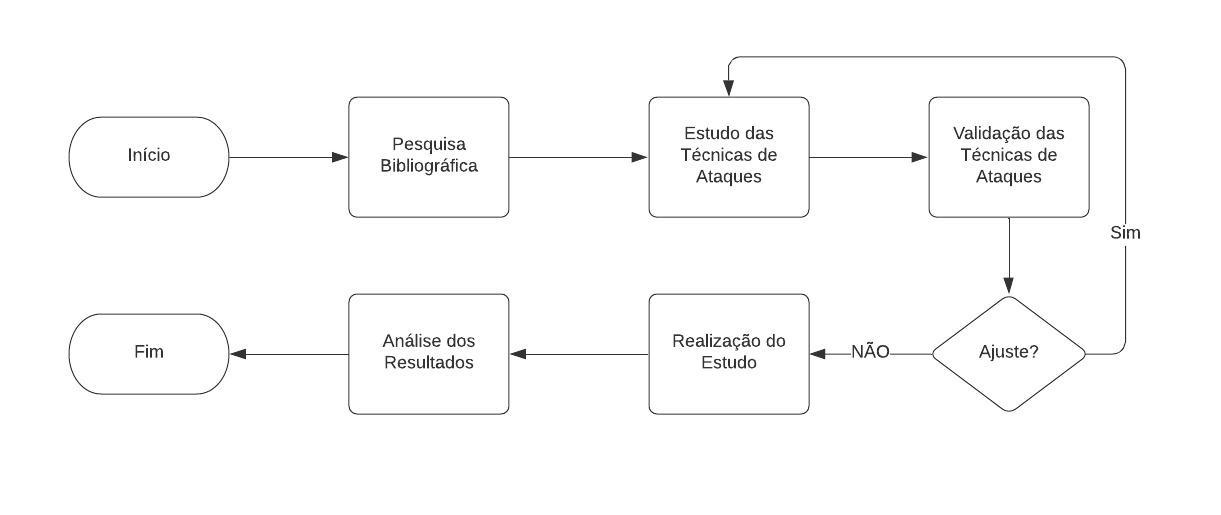
\includegraphics[width=1.0\textwidth]{fluxogramaD.jpeg}
	\caption{Metodologia do projeto}
\end{figure}

\textbf{Pesquisa bibliográfica:}
Essa é a primeira fase, nela será feito um levantamento com vários trabalhos para identificar problemas. A pesquisa também serve para coletar informações e possivelmente métodos e métricas que possam ser usados.

\textbf{Estudo das técnicas de ataques:}
Nessa fase busca-se compreender como vai funcionar 
os ataques, escolhendo algoritmos específicos e ferramentas para obtenção de resultados. Como por exemplo, é necessário uma ferramenta para realizar o \textit{sniffing} dos protocolos.

\textbf{Validação das técnicas de ataques:}
Nesta etapa, será feito um estudo e releitura das técnicas propostas, visando utilizar as mais novas tecnologias, para uma obtenção de resultados
mais satisfatórios.  

\textbf{Realização do estudo:}
Após escolhido os parâmetros, métodos e métricas desejadas o modelo do estudo pode ser gerado. Nesse projeto serão escolhidas redes sem fio que possibilitam ataques ativos e ataques passivos. 

\textbf{Análise dos resultados:}
É a última fase do projeto. Nessa fase os resultados
obtidos serão analisados e serão feitas conclusões acerca deles. Os resultados normalmente são apresentados com gráficos ou tabelas.

Por fim, a Tabela \ref{tab:tabela} apresenta o cronograma planejado para execução do projeto.
% Please add the following required packages to your document preamble:
% \usepackage{graphicx}
\begin{table}[h]
\caption{Cronograma de atividades.\label{tab:tabela}}
\resizebox{\textwidth}{!}{%
\begin{tabular}{|c|c|c|c|c|c|}
\hline
Atividades                      & Mês 1 - 2 & Mês 3 - 6 & Mês 7 - 8 & Mês 9 - 10 & Mês 11 - 12 \\ \hline
Pesquisa bibliográfica          & X         & X         &           &            &             \\ \hline
Desenvolver técnicas de ataques & X         & X         &           &            &             \\ \hline
Realizar testes das técnicas    &           & X         & X         &            &             \\ \hline
Escrita de artigos científicos  &           &           & X         & X          &             \\ \hline
Redação da monografia           &           &           & X         & X          &             \\ \hline
Defesa da monografia            &           &           &           &            & X           \\ \hline
\end{tabular}%
}
\end{table}


% ----------------------------------------------------------
% Referências bibliográficas
% ----------------------------------------------------------

\bibliography{abntex2-modelo-references}

\begin{figure} [!hbt] 
\centering
	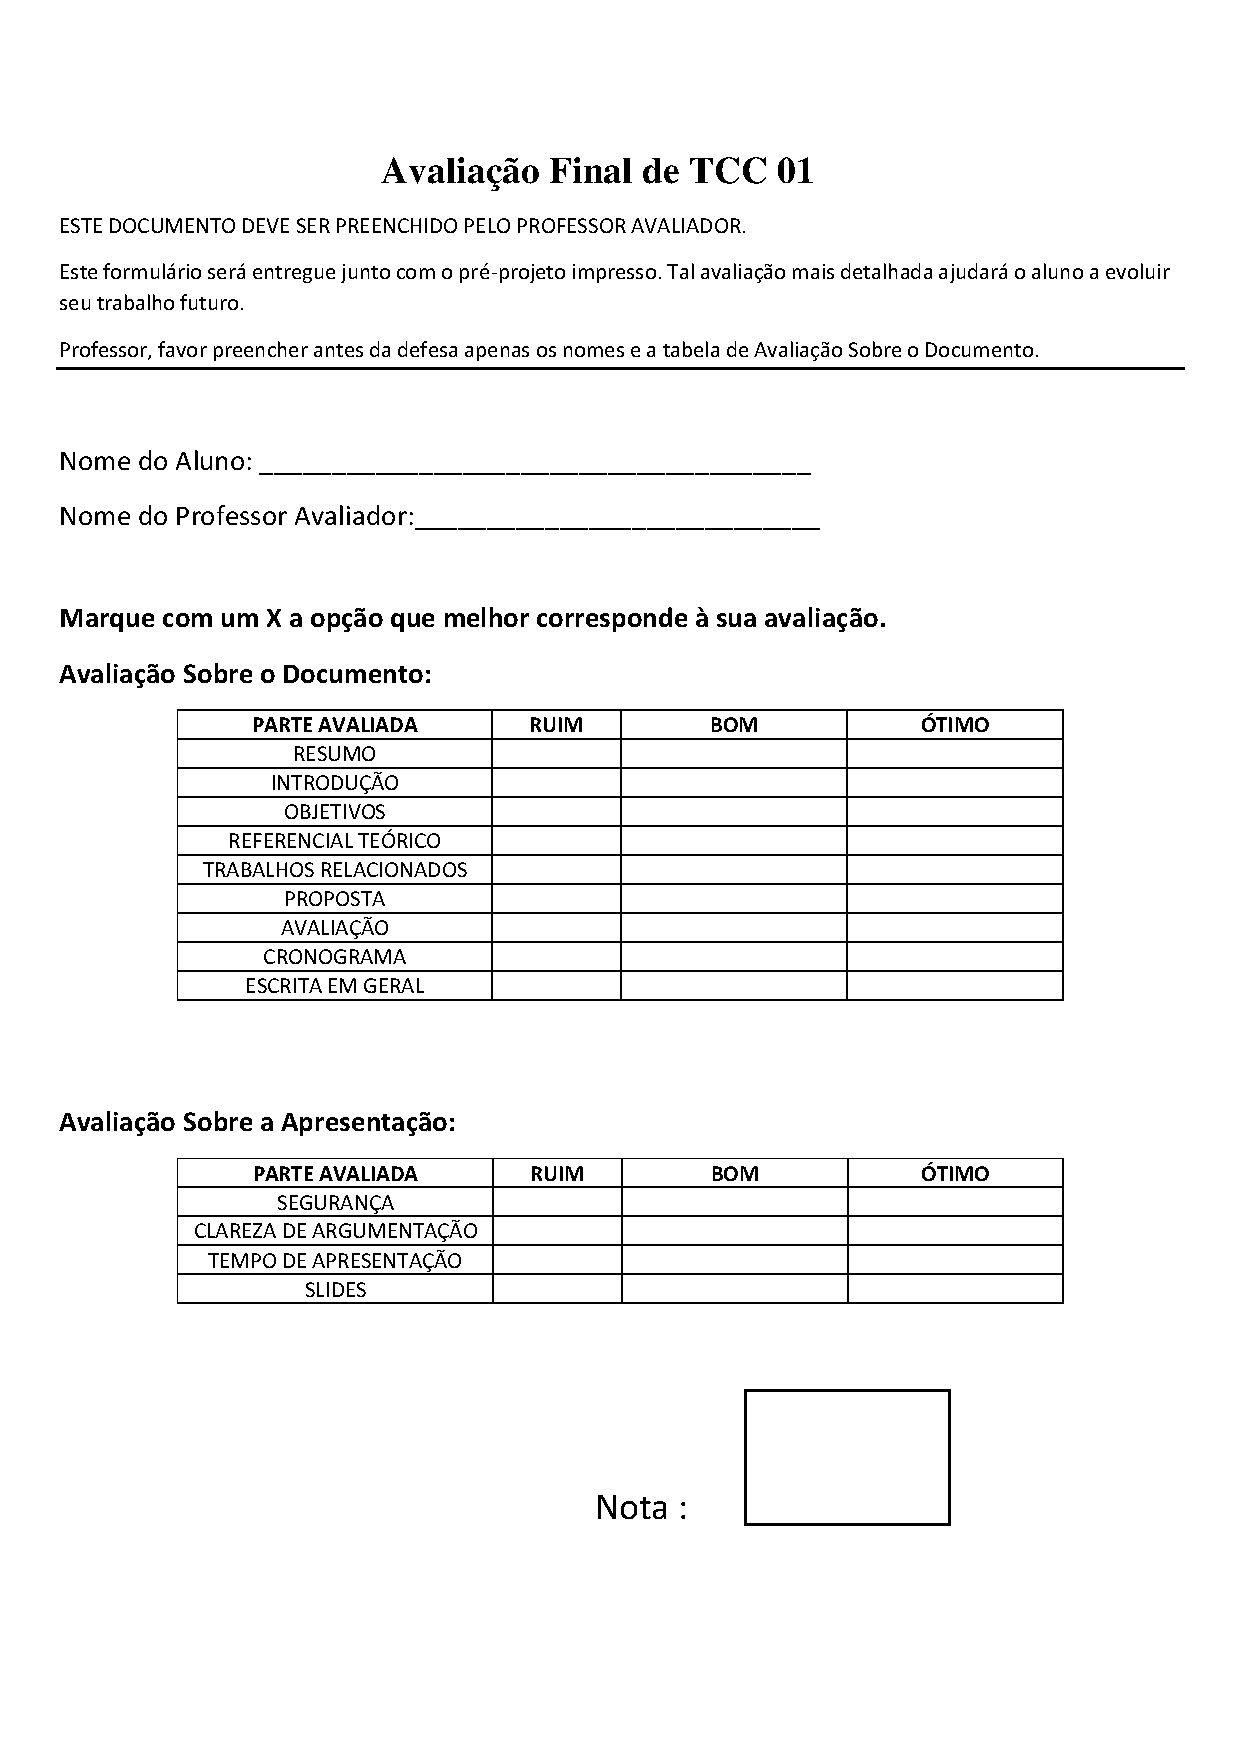
\includegraphics[width=0.95\textwidth]{formulario}
\end{figure}

\end{document}

